\documentclass[12pt,letterpaper]{article}
\usepackage{graphicx,textcomp}
\usepackage{natbib}
\usepackage{setspace}
\usepackage{fullpage}
\usepackage{color}
\usepackage[reqno]{amsmath}
\usepackage{amsthm}
\usepackage{fancyvrb}
\usepackage{amssymb,enumerate}
\usepackage[all]{xy}
\usepackage{endnotes}
\usepackage{lscape}
\newtheorem{com}{Comment}
\usepackage{float}
\usepackage{hyperref}
\newtheorem{lem} {Lemma}
\newtheorem{prop}{Proposition}
\newtheorem{thm}{Theorem}
\newtheorem{defn}{Definition}
\newtheorem{cor}{Corollary}
\newtheorem{obs}{Observation}
\usepackage[compact]{titlesec}
\usepackage{dcolumn}
\usepackage{tikz}
\usetikzlibrary{arrows}
\usepackage{multirow}
\usepackage{xcolor}
\newcolumntype{.}{D{.}{.}{-1}}
\newcolumntype{d}[1]{D{.}{.}{#1}}
\definecolor{light-gray}{gray}{0.65}
\usepackage{url}
\usepackage{listings}
\usepackage{color}

% from lshort.pdf
\usepackage{verbatim}


\definecolor{codegreen}{rgb}{0,0.6,0}
\definecolor{codegray}{rgb}{0.5,0.5,0.5}
\definecolor{codepurple}{rgb}{0.58,0,0.82}
\definecolor{backcolour}{rgb}{0.95,0.95,0.92}

\lstdefinestyle{mystyle}{
	backgroundcolor=\color{backcolour},   
	commentstyle=\color{codegreen},
	keywordstyle=\color{magenta},
	numberstyle=\tiny\color{codegray},
	stringstyle=\color{codepurple},
	basicstyle=\footnotesize,
	breakatwhitespace=false,         
	breaklines=true,                 
	captionpos=b,                    
	keepspaces=true,                 
	numbers=left,                    
	numbersep=5pt,                  
	showspaces=false,                
	showstringspaces=false,
	showtabs=false,                  
	tabsize=2
}
\lstset{style=mystyle}
\newcommand{\Sref}[1]{Section~\ref{#1}}
\newtheorem{hyp}{Hypothesis}

\title{Problem Set 1}
\date{Due: October 3, 2021}
\author{Imelda Finn, 22334657}

\begin{document}
	\maketitle

\begin{comment}	
	\section*{Instructions}
	\begin{itemize}
		\item Please show your work! You may lose points by simply writing in the answer. If the problem requires you to execute commands in \texttt{R}, please include the code you used to get your answers. Please also include the \texttt{.R} file that contains your code. If you are not sure if work needs to be shown for a particular problem, please ask.
		\item Your homework should be submitted electronically on GitHub in \texttt{.pdf} form.
		\item This problem set is due before 8:00 on Friday October 3, 2021. No late assignments will be accepted.
		\item Total available points for this homework is 100.
	\end{itemize}
\end{comment}


	\vspace{1cm}
	\section*{Question 1 (50 points): Education}
	
	\emph{A school counselor was curious about the average of IQ of the students in her school and took a random sample of 25 students' IQ scores. The following is the data set:}\\
	\vspace{.5cm}
	
	\lstinputlisting[language=R, firstline=38, lastline=39]{PS01_answersIF.R}  
	
	\vspace{.5cm}
	
	\begin{enumerate}
		\item \emph{Find a 90\% confidence interval for the average student IQ in the school.}\\
		  \begin{verbatim}
		  # calculate sample statistics
      # capture the number of observations 
      n <- length(iqData)

      # calculate mean
      iqSum <- sum(iqData)           # sum of IQ scores
      iqMean <-iqSum / n             # mean IQ score for sample

      # calculate variance and standard deviation
      iqVar <- sum((iqData - iqMean)^2)/(n-1) 
      iqSD <-sqrt(iqVar)
      
      iqse <- iqSD / sqrt(n)         # standard error of sample
      
		  \end{verbatim}
      
      The code for the t-test at 90\% is:\footnote{t.val = 1.71}
      
      \begin{verbatim}
      t.val <- qt(alphaVal/2, df = n-1, lower.tail = FALSE)

      CI_lower <- iqMean - t.val * iqse 
      CI_upper <- iqMean + t.val * iqse 

      \end{verbatim}
      The result was:
      
      Our Confidence interval for the IQ of the students in the sample is: 
       
       $93.96 <$ mean IQ $< 102.92$ 
       
       with a confidence level of 90\%.
       \footnote{A Z-test gave a  90\% CI of $94.13 < \mu < 102.75$.}
      
      
		\item \emph{Next, the school counselor was curious  whether  the average student IQ in her school is higher than the average IQ score (100) among all the schools in the country.}\\ 
		\noindent \emph{Using the same sample, conduct the appropriate hypothesis test with $\alpha=0.05$.}
		
		\begin{enumerate}
		    \item The number of observations is 25, which isn't ideal for t-test statistics
		    (we would prefer at least 30 observations).  The data isn't really random, as all are students from the same school.
		    
		    \item H$_0$: the average IQ score in the sample is less than the population average
		    ie $\mu_O \le \mu$
		    \item H$\alpha$: the average IQ score in the sample is greater than the population average  ie $\mu_O > \mu$
		    \item Calculate test statistic  
		    \[TS = \frac{\bar{Y}  - \mu_0 }{\sigma_{\bar{Y}}}\]
		    \item  Calculate p-value 
		    \[p = Pr( Z \le - |\frac{\bar{Y}  - \mu_O }{\sigma_{\bar{Y}}} |)\]
		    
		    \item if p $\le$ $\alpha=0.05$, we reject the null hypothesis
		    
		  \end{enumerate}
		  
		  \noindent

		  \begin{verbatim} 

  		  # Test our hypothesis
        alphaVal <- 0.05
        popMean <- 100
        #get test statistic
        testStatistic <- (iqMean - popMean) / iqse
                  
        pValue <- pnorm(-abs(testStatistic))

        # calculate t-test p-value 
        t_pValue <- pt(abs(testStatistic), df = n-1, lower.tail = FALSE)


		  \end{verbatim} 

      \textbf{Results}

		  p-value for normal distribution is 0.276

      \begin{tabular}{r|r|r}
          t & df  & p-value\\
 -0.5957439 &24 &0.2784617\\
      \end{tabular}
        The p-value is greater than 5\%, so we cannot reject the null hypothesis. 
        The data does not support the suggestion that the school IQ scores are greater than the 
        population average.


	\end{enumerate}
	
	\newpage
	
	\section*{Question 2 (50 points): Political Economy}
	
	\noindent Researchers are curious about what affects the amount of money communities spend on addressing homelessness. The following variables constitute our data set about social welfare expenditures in the USA. \\
	\vspace{.5cm}


	\begin{tabular}{r|l}
		\texttt{State} &\emph{50 states in US} \\
		\texttt{Y} & \emph{per capita expenditure on shelters/housing assistance in state}\\
		\texttt{X1} & \emph{per capita personal income in state} \\
		\texttt{X2} & \emph{Number of residents per 100,000 that are "financially insecure" in state}\\
		\texttt{X3} & \emph{Number of people per thousand residing in urban areas in state} \\
		\texttt{Region} & \emph{1=Northeast, 2= North Central, 3= South, 4=West} \\
	\end{tabular}
	
	\vspace{.5cm}
%	\noindent Explore the \texttt{expenditure} data set and import data into \texttt{R}.
	\vspace{.5cm}
	\lstinputlisting[language=R, firstline=173, lastline=173]{PS01_answersIF.R}  
	\vspace{.5cm}
	\begin{itemize}
		
		\item
		%Please plot the relationships among \emph{Y}, \emph{X1}, \emph{X2}, and \emph{X3}? What are the correlations among them (you just need to describe the graph and the relationships among them)?
		In Figure~\ref{pairs}, there appears to be some positive correlation between
		the per capita expenditure on Shelters$/$Housing Assistance (SHA) and each of the three
		numerical variables.  In each case, an increase in the response variable accompanies an
		increase in the candidate explanatory variable.  
		
		\begin{figure}
		  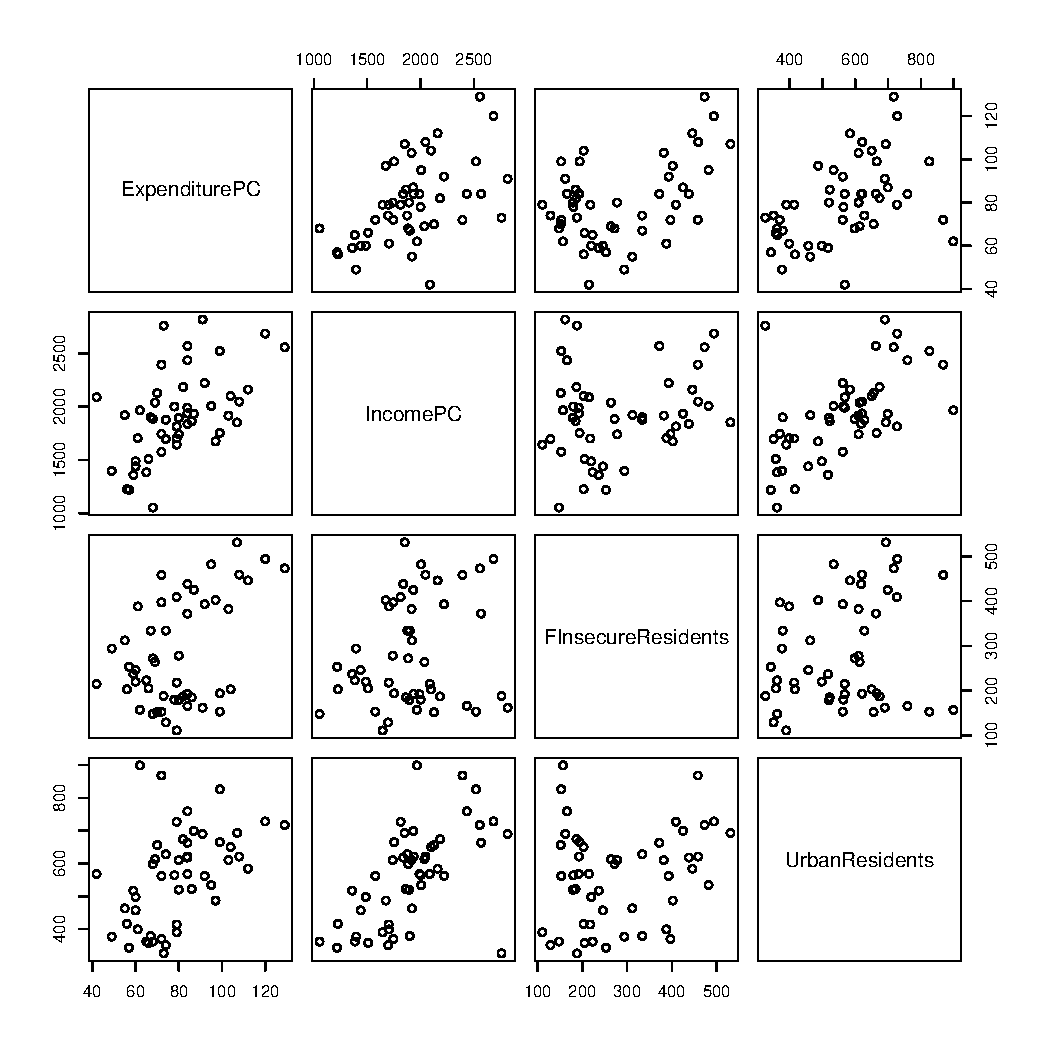
\includegraphics{expenditure_pairs.pdf}
		  \caption{Pair-wise comparison of expenditure variables}\label{pairs}
		\end{figure}
		
		The weakest relationship is between SHA expenditure and the number of residents 
		who are financially insecure.  When looked at in more detail,  Figure~\ref{y_x2} shows that
		there is a negative correlation between the two variables (ie SHA expenditure per capita
		decreases as the number of financially insecure residents increases) until $X2$ reaches
		approximately 300 per 100,000;
		after that point, the values increases are positively correlated.  (line fitted using:
		\verb|`geom_smooth()` using method = 'loess' and formula 'y ~ x'|)


		The income per capita shows some correlation with expenditure and with the number of
		urban residents, but not with financially insecure residents.  Similarly, the plot of
		urban residents against financially insecure residents appears to be uniformly distributed,
		(i.e. uncorrelated), while expenditure and income both increase with the increase in urban
		population.  
		Figure~\ref{y_x3} shows that the slope of the line relating expenditure on SHA to the urban
		population turns negative after $X3$ reaches approximately 750 per 1,000, however there are
		very few data points in this region of the plot.

		\begin{figure}
		  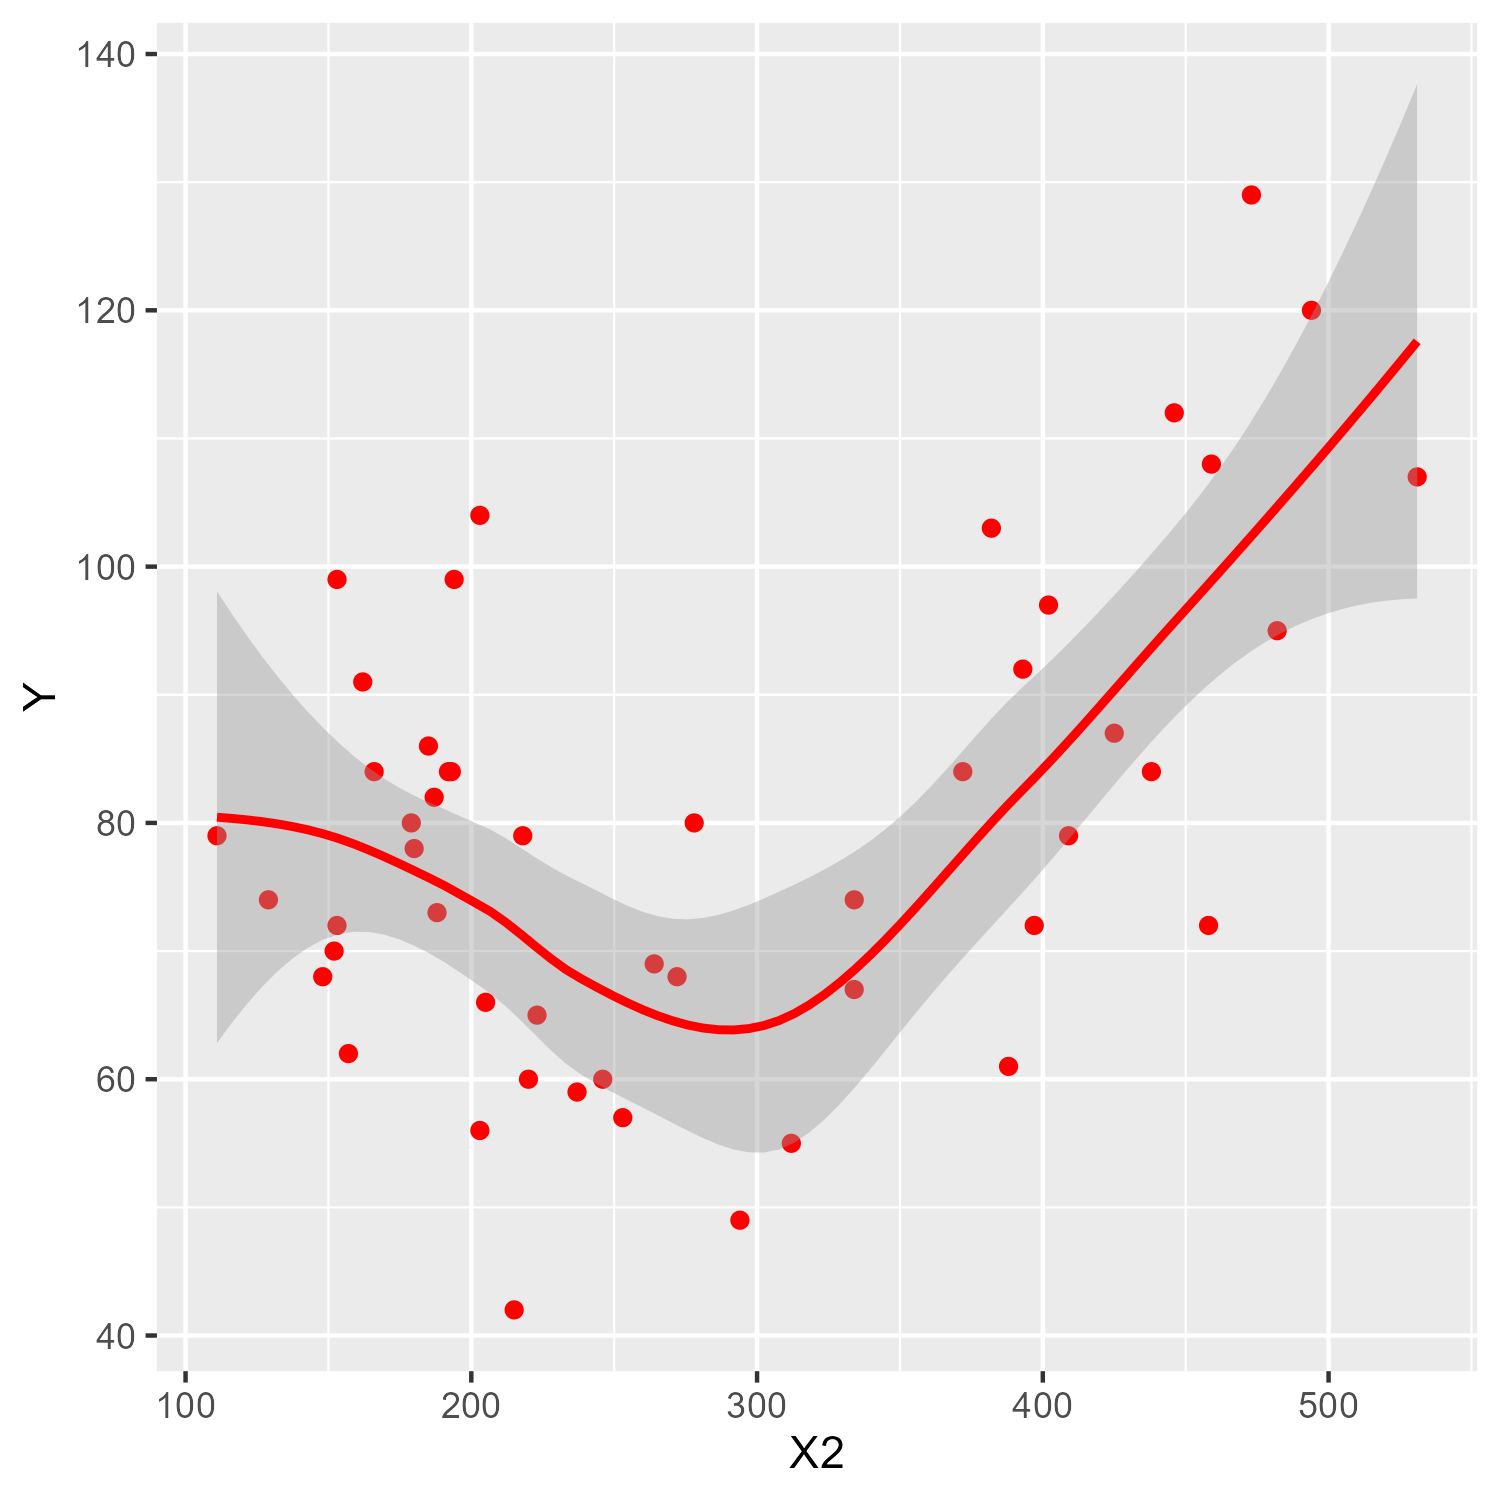
\includegraphics[width=10cm]{y_x2.png}
		  \caption{Relationship between expenditure on SHA and financially insecure 
		  population }\label{y_x2}
		  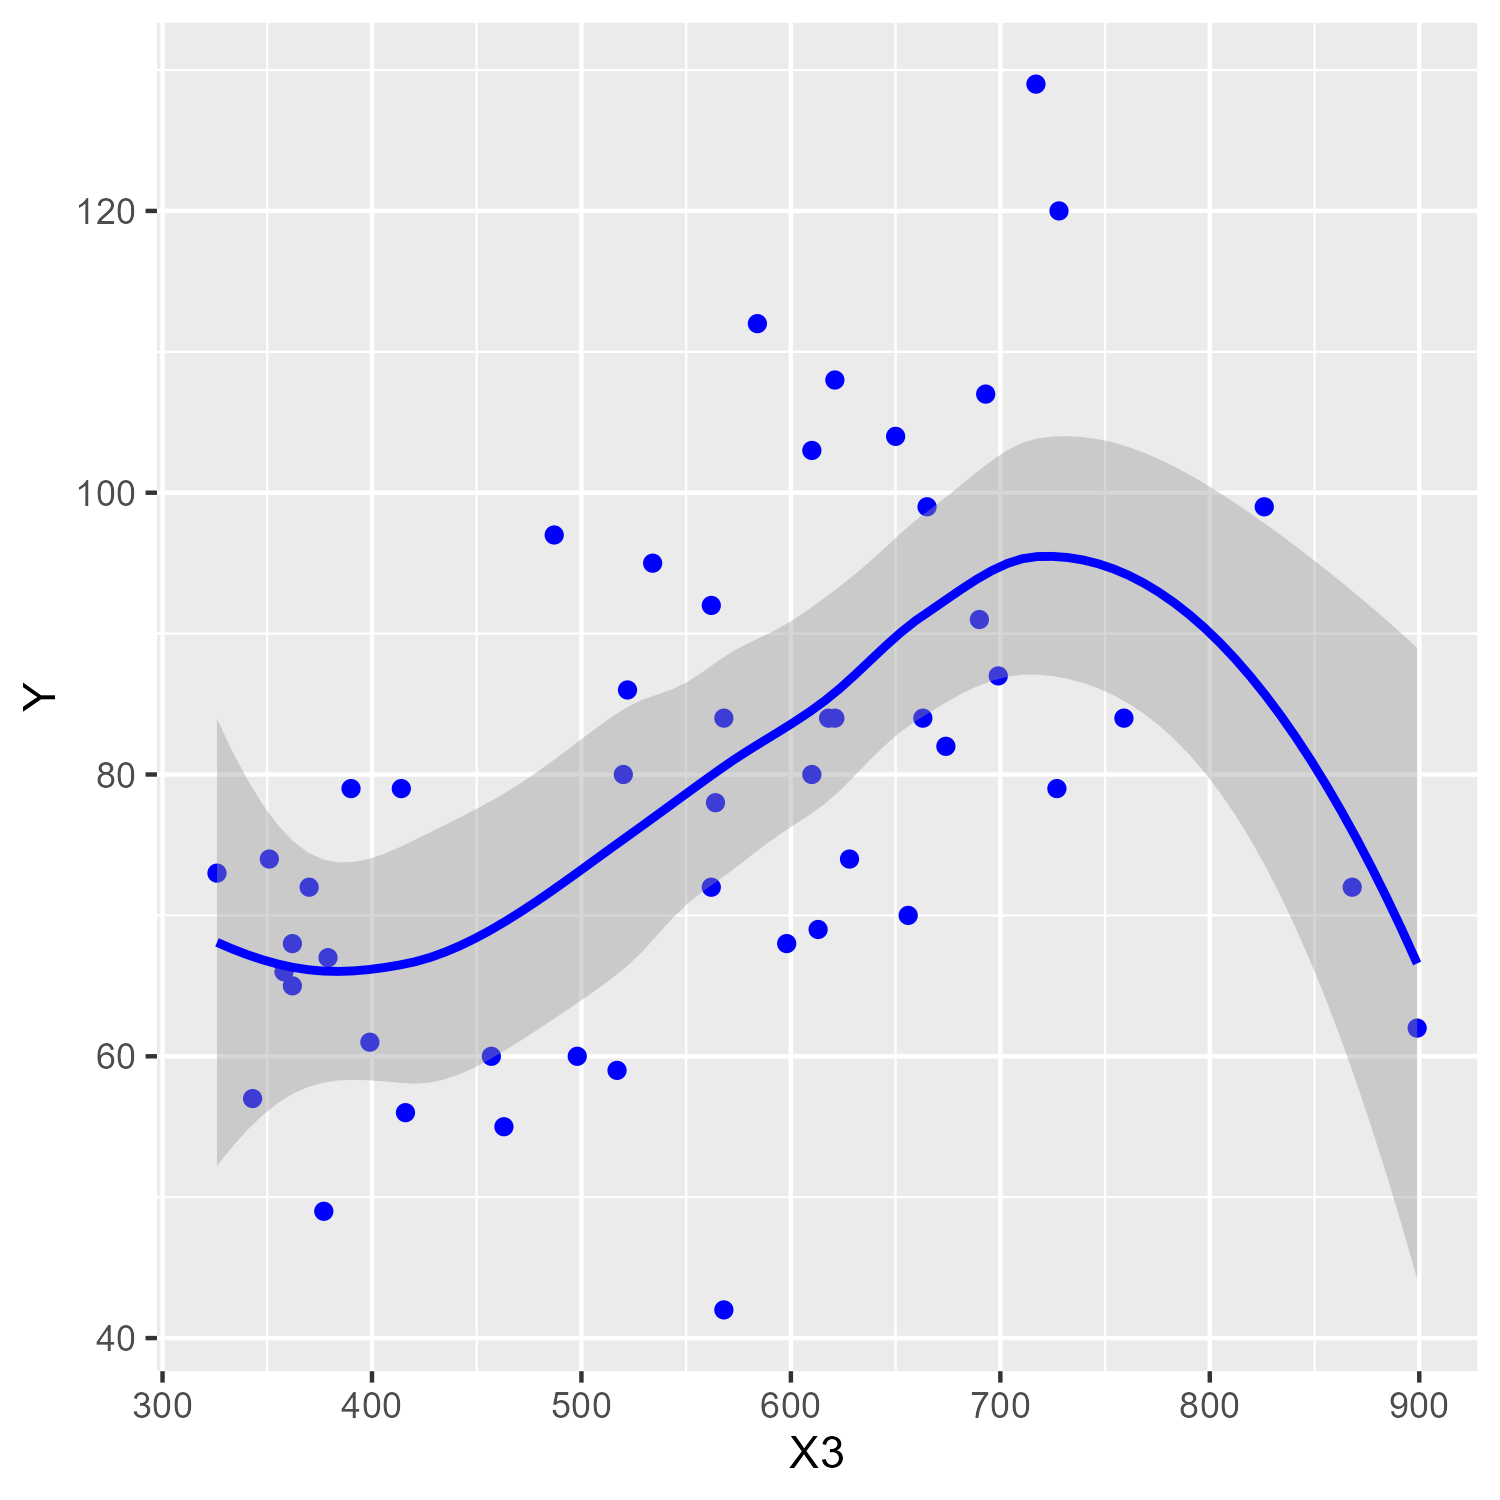
\includegraphics[width=10cm]{y_x3.png}
		  \caption{Relationship between expenditure on SHA and urban population }\label{y_x3}
		\end{figure}
		
		
		\vspace{.5cm}
		\item
		\clearpage
		%Please plot the relationship between \emph{Y} and \emph{Region}? On average, which region has the highest per capita expenditure on housing assistance?
		The relationship between expenditure on SHA and region is shown in Figure~\ref{regions}

    \begin{figure}
      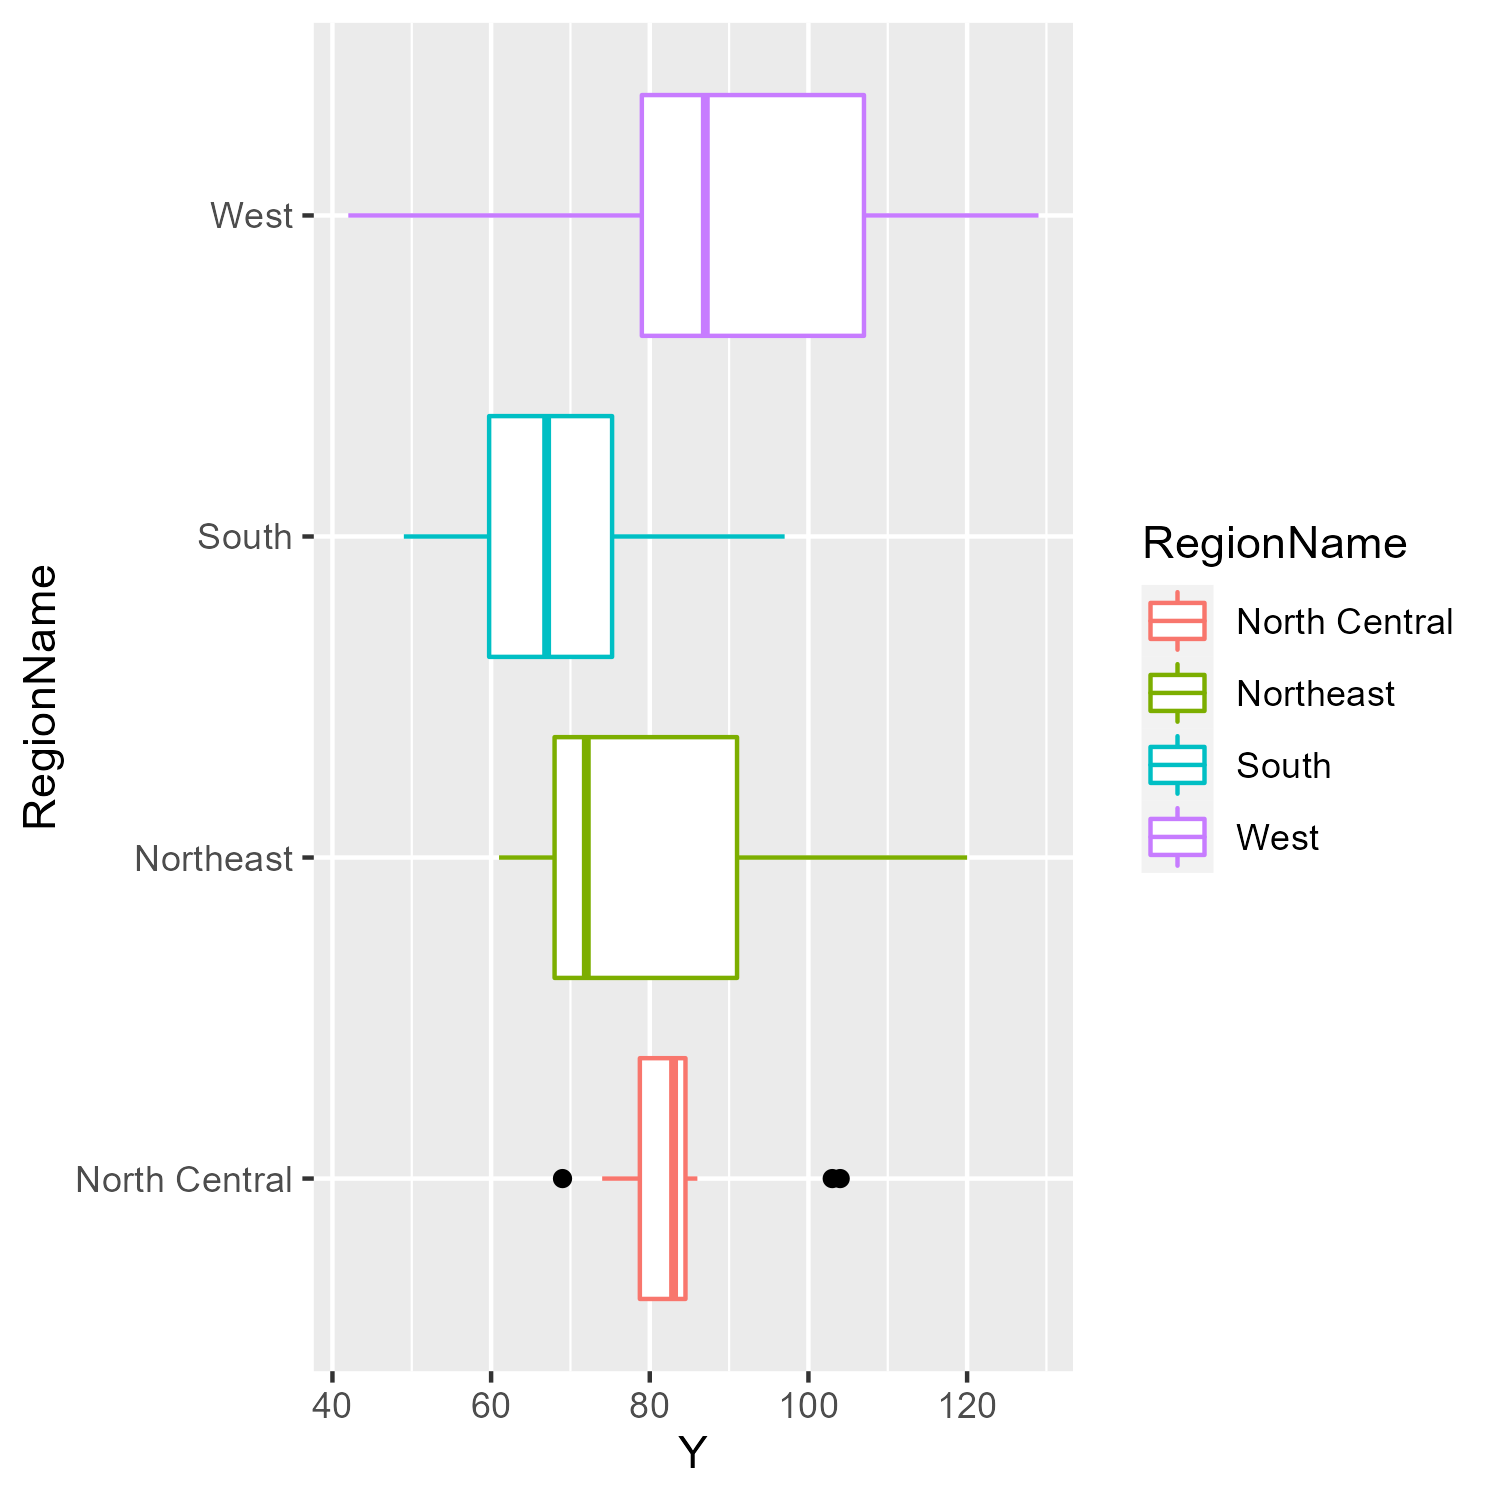
\includegraphics[width=9.5cm]{region_boxplot.png}
    	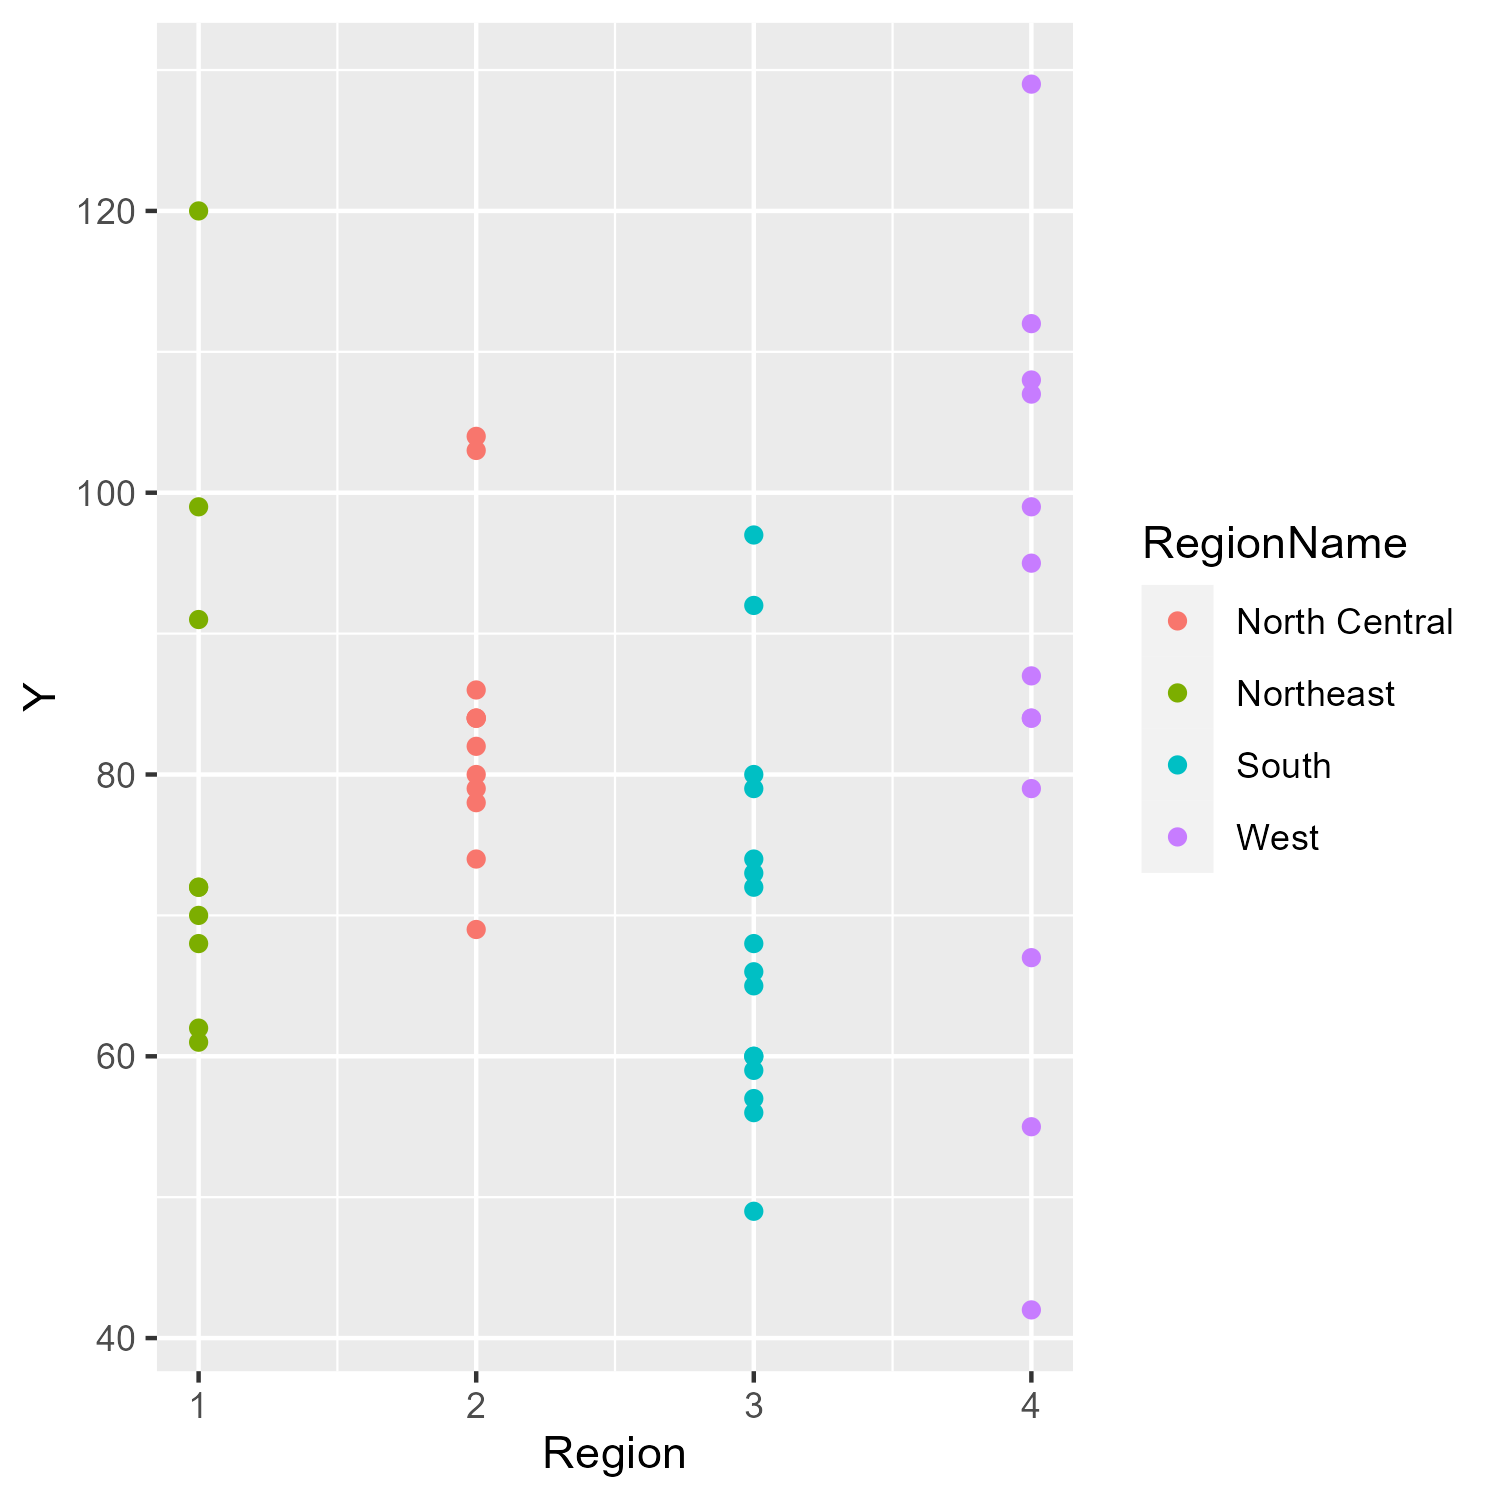
\includegraphics[width=9.5cm]{region_y.png}
      \caption{SHA expenditure by geographical region}\label{regions}
    \end{figure}
    
%    The West region has the greatest spread of Y values, North Central has the least.
		\begin{verbatim}
		  regional_mean_table <-expenditure %>% # Tidyverse method for grouping
        group_by(Region) %>%
        summarise(mean = round(mean(Y), 2))
		\end{verbatim}
    
    
% Table created by stargazer v.5.2.3 by Marek Hlavac, Social Policy Institute. E-mail: marek.hlavac at gmail.com
% Date and time: Mon, Sep 26, 2022 - 01:00:44
\begin{table}[!htbp] \centering 
  \caption{} 
  \label{} 
\begin{tabular}{@{\extracolsep{5pt}}lccccc} 
\\[-1.8ex]\hline 
\hline \\[-1.8ex] 
Statistic & \multicolumn{1}{c}{N} & \multicolumn{1}{c}{Mean} & \multicolumn{1}{c}{St. Dev.} & \multicolumn{1}{c}{Min} & \multicolumn{1}{c}{Max} \\ 
\hline \\[-1.8ex] 
mean & 4 & 80.214 & 8.193 & 69.188 & 88.308 \\ 
\hline \\[-1.8ex] 
\end{tabular} 
\end{table}  


    The West region has the highest average per capita spending (\$88.31) on Shelters$/$Housing Assistance
    (Table~\ref{tab:region_mean}).

		
		\vspace{.5cm}
%----------------------------------------------------------------------------------

		\item
%		Please plot the relationship between \emph{Y} and \emph{X1}? Describe this graph and the relationship. Reproduce the above graph including one more variable \emph{Region} and display different regions with different types of symbols and colors.
    The graph of income per capita (X1, \$) against expenditure on SHA per capita (Y, \$) appears
    to show a positive correlation between the two variables, i.e. it suggests that higher
    pc income could be a predictor for higher spending on housing assistance (Figure~\ref{y_x1}).

    \begin{figure}
      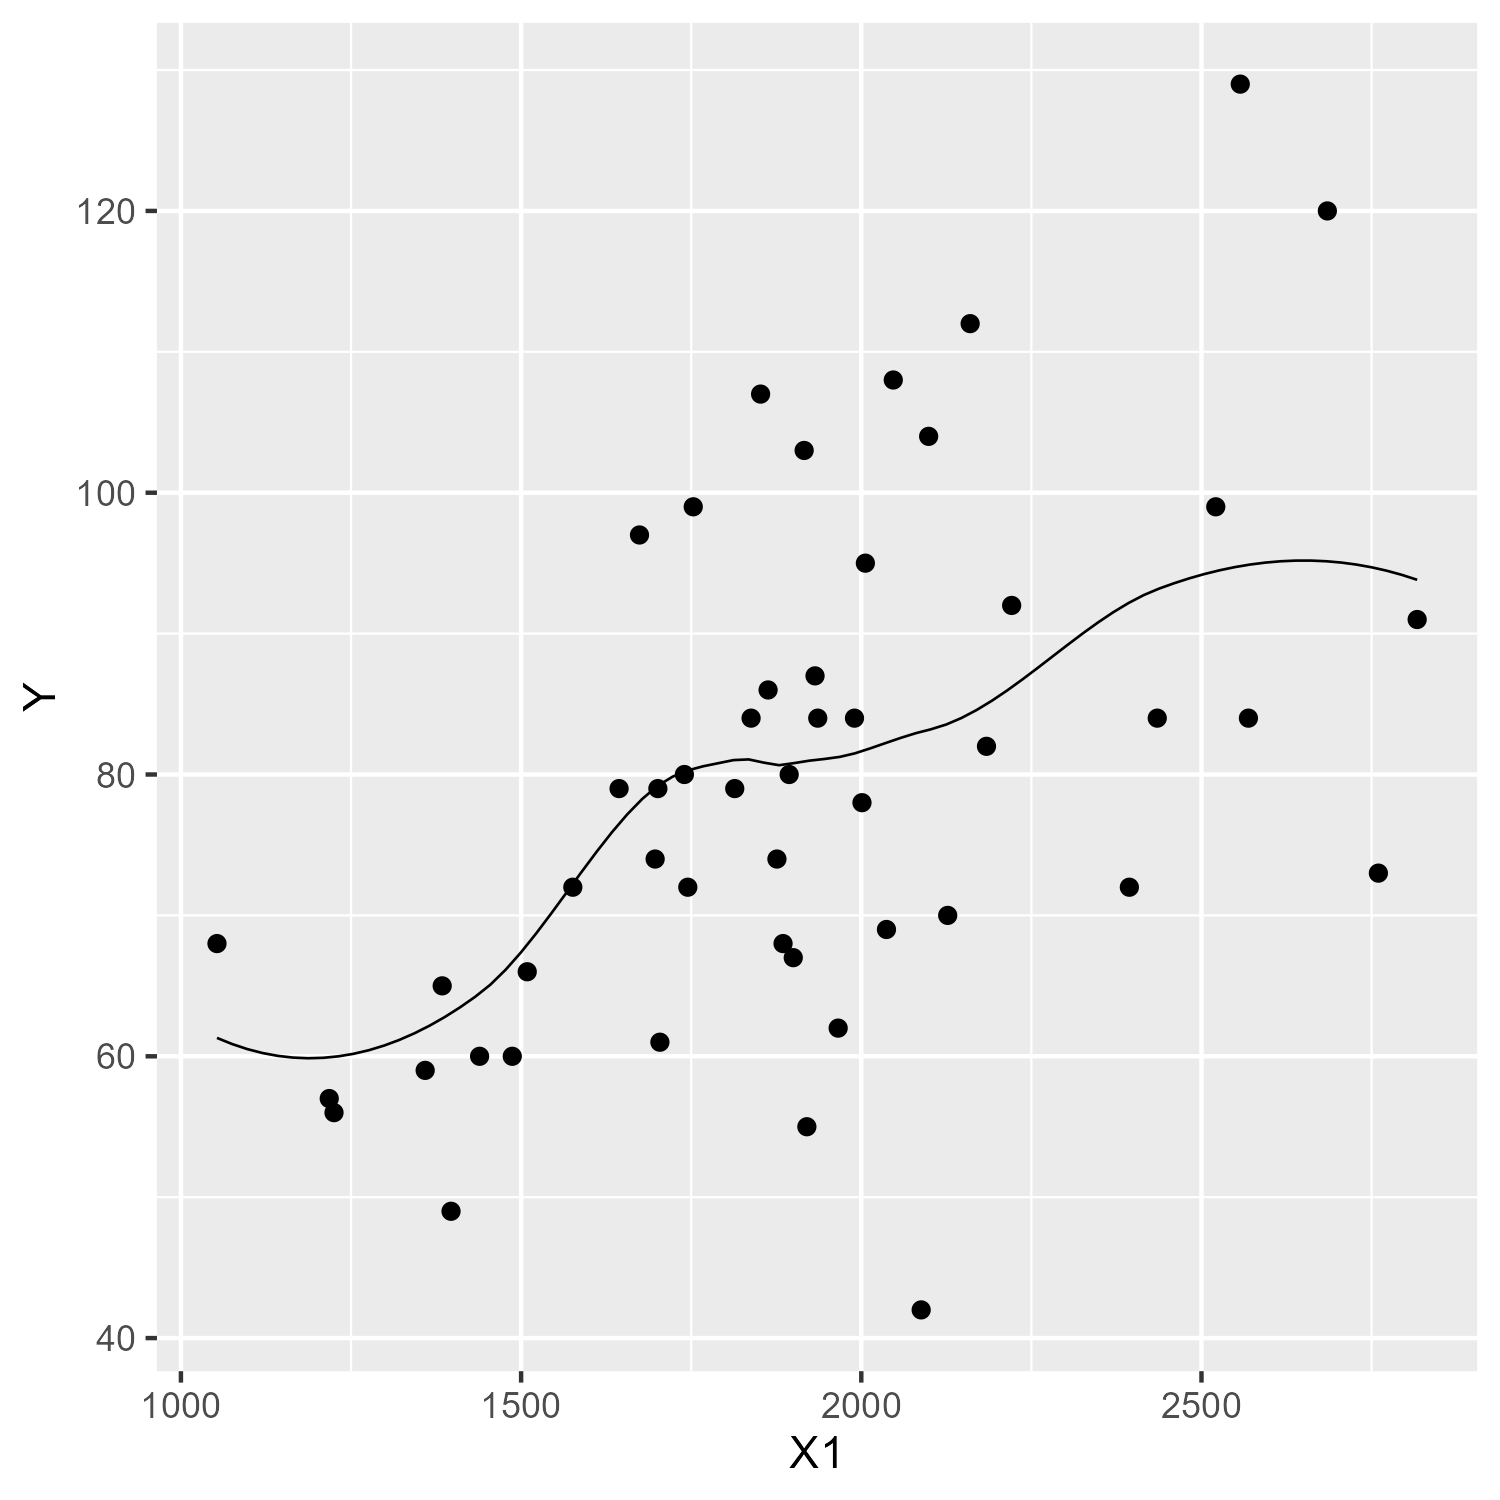
\includegraphics[width=16cm]{y_x1.png}
      \caption{Income vs SHA expenditure, per capita}\label{y_x1}
    \end{figure}


    When the data is subdivided by region the relationship between the variables is much less
    convincing.  The individual regions show clear differences between the interaction of the 
    two values - North Central and South show no positive correlation; in the Northeast and West
    it is possible that some kind of relationship exists, but it's not consistent
    (Figure~\ref{x1_regions}).
    
    The apparent relationship when the data are combined clearly masks underlying differences
    between the regions.

    \begin{figure}
      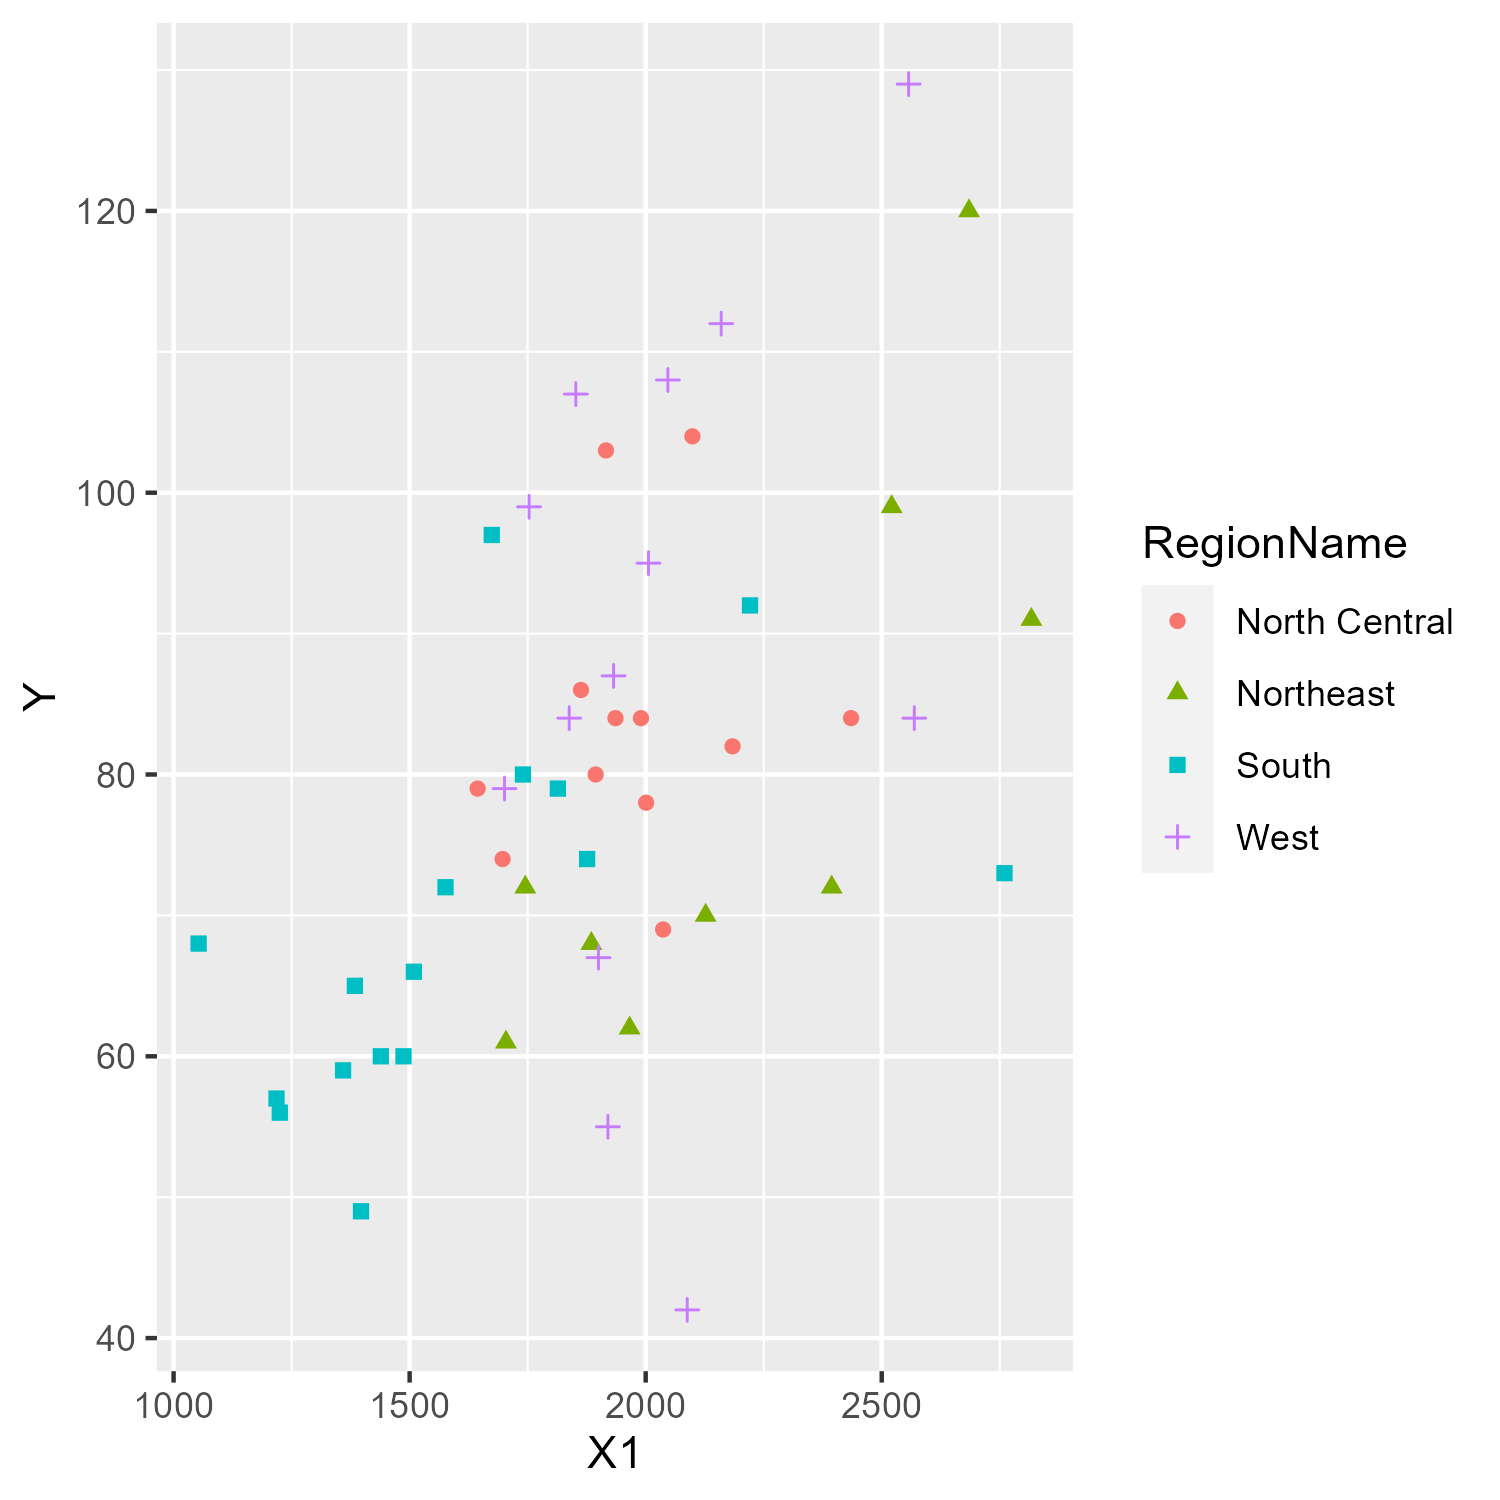
\includegraphics[width=9.5cm]{y_x1_region.png}
    	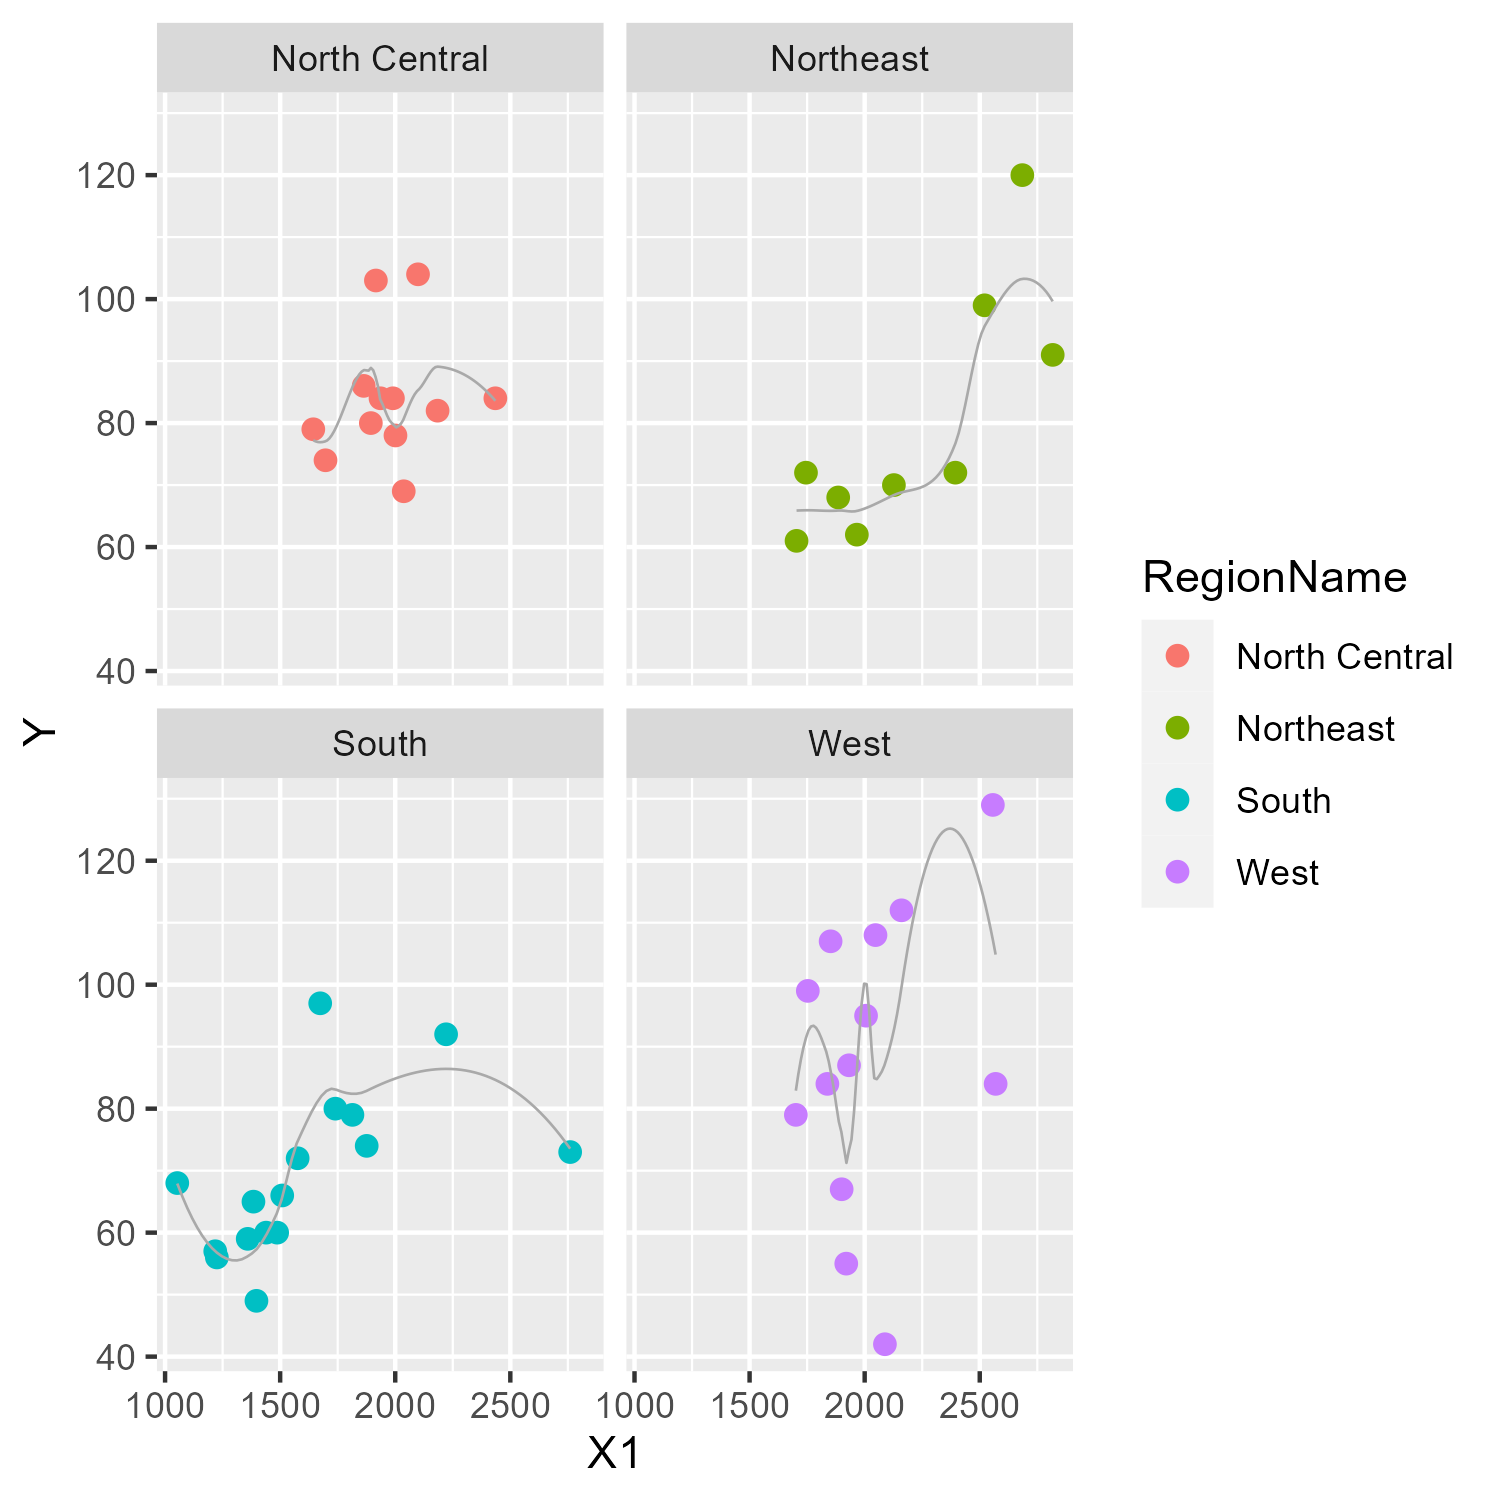
\includegraphics[width=9.5cm]{y_x1_region_facet.png}
      \caption{Income per capita vs SHA expenditure, by Region}\label{x1_regions}
    \end{figure}

	\end{itemize}

\clearpage	
\newpage

	\appendix{Appendix - R code}
  \lstinputlisting[language=R]{PS01_answersIF.R}
\end{document}
